\subsection{Documentazione}
\subsubsection{Scopo}
Tutti i processi e le attività di sviluppo devono essere documentate. Questa sezione ha lo scopo di definire le norme, le convenzioni e la struttura organizzativa riguardanti la documentazione, oltre che la definizione degli strumenti necessari alla sua stesura.
\subsubsection{Aspettative}
\begin{itemize}
	\item Avere una chiara struttura per i documenti, in modo da ottenere un risultato uniforme alla fine del loro ciclo di vita;	
	\item Avere norme e convenzioni ben precise che coprono tutti gli aspetti della stesura di un documento, in modo che tutti i membri di \Gruppo{} possano lavorare senza dover interpellare il gruppo per prendere decisioni riguardo un aspetto generico.
\end{itemize}
\subsubsection{Descrizione}
La documentazione è un processo utile a registrare le informazioni prodotte da una specifica attività del ciclo di vita. Il processo contiene un insieme di attività che pianificano, progettano, sviluppano, producono, modificano, distribuiscono e mantengono i documenti necessari a tutti gli \glo{stakeholder}.
\subsubsection{Istanziazione del processo}
\paragraph{Ciclo di vita di un documento}
\begin{figure}[!htb]
   %\begin{minipage}{0.6\textwidth}
     \centering
     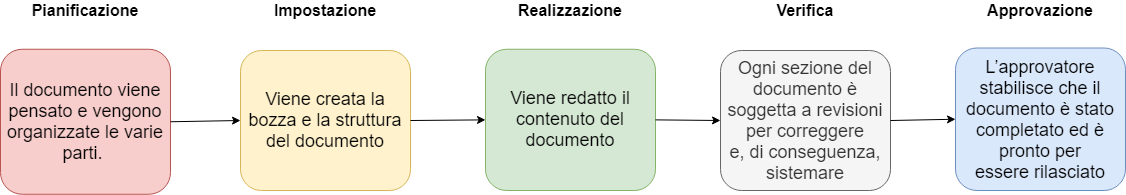
\includegraphics[scale=0.45]{Images/DocumentLifeCycle.png}
     \caption{Fasi del ciclo di vita di un documento}
   %\end{minipage}
\end{figure}

\paragraph{Sviluppo e design}  \label{pdp}

\textbf{Template}\\
Il gruppo ha deciso di creare un template con l'utilizzo di \LaTeX{}, grazie al quale viene standardizzata la struttura dei documenti. In questo modo i componenti del gruppo si occupano unicamente di redigere il contenuto dei singoli testi velocizzando la stesura degli stessi. Più precisamente, nel template vengono definite la prima pagina, la struttura del registro delle modifiche e l'indicizzazione delle sezioni e sottosezioni. \\ \mbox{}

\textbf{Struttura del documento}\\
Ogni documento è formato da diverse sezioni, ognuna definita dal proprio file \LaTeX. La parte principale è chiamata "\textit{nomedoc}.tex" (dove \textit{nomedoc} indica il nome del documento) ed ha il compito di includere le seguenti componenti:
\begin{itemize}
	\item I file \LaTeX{} delle sezioni, che contengono il contenuto del testo vero e proprio. Se presenti numerose sottosezioni in una sezione, quest'ultima deve includere i file di tutte le varie sottosezioni;
	
	\item Il registro delle modifiche, che contiene una lista delle modifiche effettuate al documento così da renderle tracciabili;
	
	\item "String.tex", che contiene una serie di comandi \LaTeX{} personalizzati che facilitano la scrittura di parole frequentemente utilizzate;
	
	\item "Comandi.tex", che contiene una serie di comandi \LaTeX{} personalizzati, diversi per ogni documento.
\end{itemize}

\mbox{}

\textbf{Prima pagina}\\
La prima pagina di un documento è formata da:
\begin{itemize}
	
	\item \textbf{Logo}: logo di \Gruppo{} posto in alto e centralizzato;
	
	\item \textbf{Progetto ed e-mail}: sotto il logo e centralizzato viene scritto il nome del progetto e la mail del gruppo \Gruppo{};
	
	\item \textbf{Titolo}: il nome del documento;
	
	\item \textbf{Informazioni sul documento}: sotto al titolo è presente una tabella con le seguenti informazioni riguardanti il documento:
	
	\begin{itemize}
		
		\item \textbf{Versione}: versione del documento;
		
		\item \textbf{Approvatori}: nomi dei componenti del gruppo che svolgono il ruolo di \glo{approvatore};
		
		\item \textbf{Redattori}: nomi dei componenti del gruppo che svolgono il ruolo di \glo{redattore};
	 	
	 	\item \textbf{Uso}: specifica il tipo di utilizzo che viene fatto di questo documento;
	 	
	 	\item \textbf{Distribuzione}: specifica a chi il documento verrà distribuito.
	 	
	\end{itemize}
	
	\item \textbf{Descrizione}: una breve descrizione del documento posta sotto la tabella.
\end{itemize}

\mbox{}

\textbf{Registro delle modifiche}\\
Il registro delle modifiche è una tabella che riporta ogni modifica effettuata al documento in cui è contenuta. Una modifica è rappresentata da una riga della tabella avente le seguenti voci:
\begin{itemize}

	\item \textbf{Versione}: versione attuale del documento;
	
	\item \textbf{Data}: data della modifica;
	
	\item \textbf{Nominativo}: il nome del \glo{redattore} della modifica e del relativo \glo{verificatore};
	
	\item \textbf{Ruolo}: il ruolo del \glo{redattore} e del \glo{verificatore} all'interno del gruppo;

	\item \textbf{Descrizione}: una breve descrizione sulla modifica effettuata.
\end{itemize}

\textbf{Indice}\\
L'indice deve elencare le sezioni in cui sono divise le diverse parti del documento, le tabelle e le immagini presenti nel documento. L'indice viene posto dopo il registro delle modifiche.

\mbox{}

\textbf{Struttura delle pagine}\\
La singola pagina di contenuto è strutturata come segue:
\begin{itemize}

	\item In alto a sinistra viene posto il logo del gruppo \Gruppo{};
	
	\item In basso a sinistra viene scritto il nome del documento;
	
	\item In basso a destra viene indicato il numero della pagina corrente sul totale delle pagine;
	
	\item Il contenuto della pagina è scritto tra l'intestazione e il piè di pagina che lo delimitano con una riga.
\end{itemize}

\mbox{}

\textbf{Verbali}\\
I \textit{Verbali} prevedono una singola stesura, dato che contengono delle decisioni che non possono essere modificate successivamente. I \textit{Verbali} contengono la prima pagina e il registro delle modifiche come gli altri documenti; viene invece omesso l'indice che il gruppo ha ritenuto poco utile data la brevità del documento.\\ Il contenuto di un \textit{Verbale} è formato da tre sezioni. La prima è l'introduzione che contiene le seguenti informazioni:
\begin{itemize}
	
	\item \textbf{Motivo della riunione}: il motivo per cui il gruppo ha deciso di organizzare un incontro e che, di conseguenza, contiene le materie che verranno discusse;
	
	\item \textbf{Luogo riunione}: il luogo dove viene svolta la riunione;
	
	\item \textbf{Data}: la data che indica quando il gruppo ha effettuato la riunione;
	
	\item \textbf{Orario di inizio}: l'ora in cui è iniziala la riunione;
	
	\item \textbf{Orario di fine}: l'ora in cui è finita la riunione;
	
	\item \textbf{Partecipanti}: l'elenco dei partecipanti al meeting.
\end{itemize}

La seconda sezione è il resoconto e deve fornire un breve riassunto di quanto discusso e delle decisioni prese. I motivi di discussione vengono riportati in un elenco dove vengono spiegati uno per volta.

Alla fine di ogni \textit{Verbale} è presente una tabella che ha la funzione di tenere traccia delle decisioni prese durante l'incontro. 

\newpage

Ogni riga della tabella prevede una descrizione molto breve della decisione e un identificativo che segue questo formato:
\begin{center}
\textbf{[Destinazione]-X.Y}
\end{center}
Dove: 

\begin{itemize}

	\item \textbf{[Destinazione]}: è \textbf{Interno}, se il verbale è interno, mentre è \textbf{Esterno}, se il verbale è esterno;
	
	\item \textbf{X.Y}: dove \textbf{X} è il numero del verbale e \textbf{Y} indica il numero della decisione all'interno del verbale.
\end{itemize}

\mbox{}

\textbf{Studio di fattibilità}\\
Il documento è suddiviso in sette sezioni, una per ogni capitolato, e ognuna di queste è composta dalle seguenti parti:
\begin{itemize}
    \item Descrizione generale;
    \item Prerequisiti e tecnologie coinvolte;
    \item Vincoli;
    \item Aspetti positivi;
    \item Aspetti critici;
    \item Conclusioni.
\end{itemize}
L'ultima parte serve ad esporre le motivazioni dello scarto o della scelta di uno specifico capitolato.\\ \mbox{} \\
\textbf{Piano di qualifica}  \\
Il \PdQ{}, redatto dal \glo{verificatore}, è suddiviso nelle seguenti parti:
\begin{itemize}
\item Qualità di processo;
\item Qualità di prodotto;
\item Specifica dei test;
\item Resoconto attività di verifica.
\end{itemize} 
\mbox{} \\
\textbf{Piano di progetto} \\
Gli amministratori e il responsabile dovranno redigere questo documento che dovrà essere seguito durante tutto il corso del progetto. È suddiviso nelle seguenti sezioni:
\begin{itemize}
    \item Analisi dei rischi;
    \item Modello di sviluppo;
    \item Pianificazione;  
    \item Preventivo;
    \item Consuntivo;
    \item Organigramma;
    \item Attualizzazione dei rischi. 
\end{itemize}
\mbox{} \\
\textbf{Analisi dei requisiti}\\
L'\textit{Analisi dei Requisiti} è formata dalle seguenti sezioni:
\begin{itemize}
	\item Descrizione generale;
	\item Casi d'uso;
	\item Requisiti.
\end{itemize}
\mbox{} \\
\textbf{Glossario}\\
Il \textit{Glossario} presenta una sezione per ogni lettera dell'alfabeto. 

\paragraph{Convenzioni}

\textbf{Nomi dei file}\\
I nomi dei file e delle cartelle seguono tutte la stessa convenzione:

\begin{itemize}

	\item I nomi dei file e delle cartelle iniziano per lettera maiuscola;
	
	\item Se il nome è composto da più parole, ognuna di queste inizia per lettera maiuscola e non è previsto alcun tipo di separazione tra una parola e l'altra.
	
\end{itemize}

Esempi corretti:

\begin{itemize}

	\item NormeDiProgetto;
	
	\item AnalisiDeiRequisiti.
	
\end{itemize}

Esempi non corretti:

\begin{itemize}

	\item Normediprogetto (non tutti le parole iniziano con lettera maiuscola);
	
	\item analisi\_dei\_requisiti (sono presenti dei caratteri separatori).
\end{itemize}

\mbox{}

\textbf{Stile di testo}
\begin{itemize}

	\item \textbf{Grassetto}: lo stile grassetto viene applicato ai termini negli elenchi puntati e ai titoli delle sezioni;
	
	\item \textbf{Corsivo}: lo stile corsivo si applica al nome del gruppo, al nome del progetto, al nome dei documenti, al nome del proponente e alle parole che hanno una particolare importanza nel contesto in cui sono inserite;
	
	\item \textbf{Nome dei documenti}: il nome dei documenti deve essere scritto in corsivo e deve iniziare per lettera maiuscola, mentre quando si fa riferimenti al documento vero e proprio viene aggiunta anche la versione, anch'essa in corsivo. Se il nome è composto da più parole, ogni parola inizia per lettera maiuscola, ad esclusione delle preposizioni.  Se il nome viene usato come titolo, questi stili non si applicano, ma il redattore deve utilizzare lo stile grassetto;
	
	\item \textbf{Link}: il testo che indica un link esterno deve essere di colore blu e sottolineato;
	
	\item \textbf{Collegamenti interni}: le parole che si riferiscono ad una parte del documento stesso vanno sottolineate.

\end{itemize}

\mbox{}

\textbf{Glossario}\\
Le norme relative al \textit{Glossario} sono:
\begin{itemize}

	\item Ogni parola del \textit{Glossario} è contrassegnata da una 'G' ad apice;
	
	\item Non vengono segnate come termini del \textit{Glossario} le parole che fanno parte di un titolo o che sono presenti nelle didascalie;
	
	\item Se un termine compare nella propria definizione all'interno del \textit{Glossario}, esso non viene contrassegnato.

\end{itemize}

\mbox{}

\textbf{Elenchi puntati e numerati}\\
Gli elenchi puntati e numerati seguono le seguenti norme:
\begin{itemize}

	\item Ogni voce inizia per lettera maiuscola;
	
	\item Ogni voce termina con ';', escludendo l'ultima che termina con '.';
	
	\item Se una voce deve descrivere un concetto, un termine o un oggetto allora esso va scritto in grassetto seguito da ':'.
\end{itemize}

I componenti del gruppo devono preferire l'utilizzo di elenchi puntati o numerati rispetto a lunghi blocchi di testo narrativi. \\

\mbox{}

\textbf{Sigle}\\
Le sigle presenti nei documenti rappresentano i ruoli dei componenti:
\begin{itemize}

	\item \textbf{RE}: responsabile di progetto;
	
	\item \textbf{AM}: amministratore;
	
	\item \textbf{AN}: analista;
	
	\item \textbf{PT}: progettista;
	
	\item \textbf{PR}: programmatore;
	
	\item \textbf{VE}: verificatore.

\end{itemize}

Nel documento \AdRv{v4.0.0-1.8} vengono usate le seguenti sigle:
\begin{itemize}
	\item \textbf{OB}: obbligatorio;
	\item \textbf{DE}: desiderabile;
	\item \textbf{OP}: opzionale.
\end{itemize}

Altri sigle che vengono utilizzate sono:
\begin{itemize}
	\item \textbf{RR}: revisione dei requisiti;
	\item \textbf{RP}: revisione di progettazione;
	\item \textbf{RQ}: revisione di qualifica;
	\item \textbf{RA}: revisione di accettazione.
\end{itemize}

\mbox{}

\textbf{Data}\\
I componenti del gruppo hanno deciso di adottare il seguente formato per la rappresentazione delle date:
\begin{center}
\textbf{DD-MM-YYYY}
\end{center}
dove \textbf{DD} indica il giorno, \textbf{MM} il mese e \textbf{YYYY} l'anno.

\paragraph{Elementi grafici}
\textbf{Tabelle}\\
Ad eccezione del registro delle modifiche, le tabelle di un documento seguono le seguenti convenzioni:
\begin{itemize}

	\item Ogni tabella ha annessa una didascalia descrittiva posizionata sotto la tabella corrispondente;
	
	\item Ogni tabella viene identificata da un numero progressivo a partire da 1, che la identifica univocamente all'interno del documento e la dichiara nell'indice delle tabelle.
\end{itemize}

\mbox{}

\textbf{Immagini}\\
Le immagini sono centralizzate e presentano un numero e una didascalia esplicativa.\\

\mbox{}

\textbf{Diagrammi}\\
Sia i diagrammi \glo{UML} che i diagrammi di \glo{Gantt} vengono riportati come immagini e quindi sono soggetti alle regole precedentemente esposte. I diagrammi \glo{UML} devono essere realizzati usando la versione 2.0 del linguaggio.

\subsubsection{Metriche}
Per poter ottenere una documentazione di buona qualità si è deciso di utilizzare le seguenti metriche.\\
Alcuni parametri per comprendere la tabella seguente:
	\begin{itemize}
		\item \textbf{Numero frasi (N\textsubscript{fr})}: numero di frasi nell'intero documento;
		\item \textbf{Numero lettere (N\textsubscript{lett})}: numero di lettere nell'intero documento;
		\item \textbf{Numero parole (N\textsubscript{par})}: numero di parole nell'intero documento.
	\end{itemize}
\renewcommand{\arraystretch}{1.5}
\renewcommand\extrarowheight{1.5pt}
\begin{longtable}{C{1.5cm} C{4.5cm} C{5.5cm} C{5cm}}
		\rowcolor{coloreRosso}
		\textcolor{white}{\textbf{Codice}} & 
		\textcolor{white}{\textbf{Nome}} & 
		\textcolor{white}{\textbf{Descrizione}} & 
		\textcolor{white}{\textbf{Formula}} \\
		\endfirsthead
	    \endfoot
	    \rowcolor{white}\caption{Metriche per la qualità dei documenti}
	    \endlastfoot
		\hline
		\textbf{MPD1} & 
		Indice Gulpease & 
		Descrive la leggibilità del documento. & 
		$ 89 + \frac{300 \cdot N_{fr} - 10 \cdot N_{lett}}{N_{par}}$ \\
		\textbf{MPD2} & 
		Errori ortografici (EO) & 
		Verifica sulla presenza di errori ortografici. & 
		- \\
\end{longtable}
\subsubsection{Strumenti}
Gli strumenti utilizzati in questo processo comprendono:
\begin{itemize}
	\item \textbf{\LaTeX{}}: linguaggio di markup per la preparazione di testi, basato sul programma di composizione tipografica \TeX{};
	\begin{center}
		\textcolor{blue}{\url{https://www.latex-project.org/}}
	\end{center}
	\item \textbf{Texmaker}: editor per scrivere codice \LaTeX{}. \Gruppo{} ha deciso di utilizzare questo editor perché gratis e poiché prevede:
\begin{itemize}
	\item Un compilatore integrato;
	\item Un visualizzatore PDF;
	\item Funzionalità interessanti come l'autocompletamento dei comandi \LaTeX{}, il controllo dell'ortografia e il \glo{code folding}.
\end{itemize}	
	\begin{center}
		\textcolor{blue}{\url{https://www.xm1math.net/texmaker/}}
	\end{center}
	\item \textbf{Draw.io}: programma per la produzione dei diagrammi \glo{UML}. Il gruppo ha scelto questo strumento perché non è richiesto scaricare alcun software per progettare un diagramma, per le funzionalità fornite e per la semplicità di utilizzo.
	\begin{center}
		\textcolor{blue}{\url{https://www.diagrams.net/}}
	\end{center}
\end{itemize}